\documentclass[a4paper,12pt]{article}
\usepackage[latin1]{inputenc} %entrada usando ISO-Latin1
\usepackage{listings}
\usepackage{color}
\usepackage{a4wide}
\usepackage{graphicx}
\usepackage{subfig}
\usepackage{wrapfig}
\usepackage{hyperref}
\usepackage{amsmath}
\usepackage{tikz}
\usetikzlibrary{shapes, arrows}
\usepackage{appendix}

\usepackage{bm, amssymb, pifont, pgfplots, multirow, float, soul, color, verbatim, indentfirst}

\newcommand{\be}{\begin{equation}}
\newcommand{\ee}{\end{equation}}

\lstset{
   breaklines=true,
   basicstyle=\ttfamily}
% \usepackage{draftwatermark}
\usepackage[figurewithin=section,tablewithin=section]{caption}
%\usepackage{subfigure}
\setcounter{secnumdepth}{4}

\pagestyle{headings}

\title{\textbf{LCLS-II System Simulations:\\Cavity Model}}
\author{LBNL LLRF Team}

\date{\today}

\begin{document}

\maketitle
\setcounter{tocdepth}{2}

\section{Cavity model}

From EM theory, we know $\vec{E}$ and $\vec{B}$ fields inside a cavity can be broken down into independent eigenmodes (independent solutions to Maxwell's equations inside a cavity or waveguide). For a 9-cell cavity, the highest $\vec{E}$ field along the cavity axis is obtained for the $\pi$-mode. Ideally we would like to only excite that mode applying the proper input signal, which is only is known from theory. However, this is hard to achieve in practice as some other modes are present due to geometrical errors in the cavity shape or further deformation due to mechanical forces that are generated.

The cavity model described here responds to a multi-cell cavity structure, with couplings to the RF source, a cavity field probe and the beam. There are two aspects to representing this problem: the complete EM field description inside the cavity and the equivalent circuit representation, where the field description is needed in order to define the equivalent circuit using simulation codes like Superfish~\cite{ref:superfish}. It is convenient to use the equivalent circuit representation in order to model the cavity behavior as well as its interactions with the RF system and the beam.

Ideally, we would like to measure the EM fields from each mode present in the cavity in order to control them appropriately. However, the best  we can do is measure the overall field in the cavity, designated here by $\vec E_{\rm probe}$. It is measured in practice using a probe antenna, and is theoretically given by

\begin{equation}
  \vec E_{\rm probe} = \sum_{\mu} \vec{V}_{\mu} /\sqrt{Q_{\rm p_{\mu}}(R/Q)_{\mu}}
  \label{eq:E_probe}
\end{equation}

\noindent where $\vec{V}_{\mu}$ is a representative measure of the energy stored in each electrical mode $\mu$, designated as mode cavity voltage, and where $Q_{\rm p_{\mu}}(R/Q)_{\mu}$ is the coupling impedance of the probe port for that mode.

Alternatively, the expression for reverse (a.k.a.~reflected) wave travelling outward from the fundamental port includes a prompt reflection term, yielding

\begin{equation}
  \vec E_{\rm reverse}=\sum_\mu \vec V_\mu / \sqrt{Q_{g_{\mu}}(R/Q)_\mu} - \vec K_g
  \label{eq:E_reverse}
\end{equation}

\noindent where $Q_{g_{\mu}}(R/Q)_\mu$ is the coupling impedance of the drive port of mode $\mu$.

\subsection{Electromagnetic eigenmode}

\begin{figure}
\centering
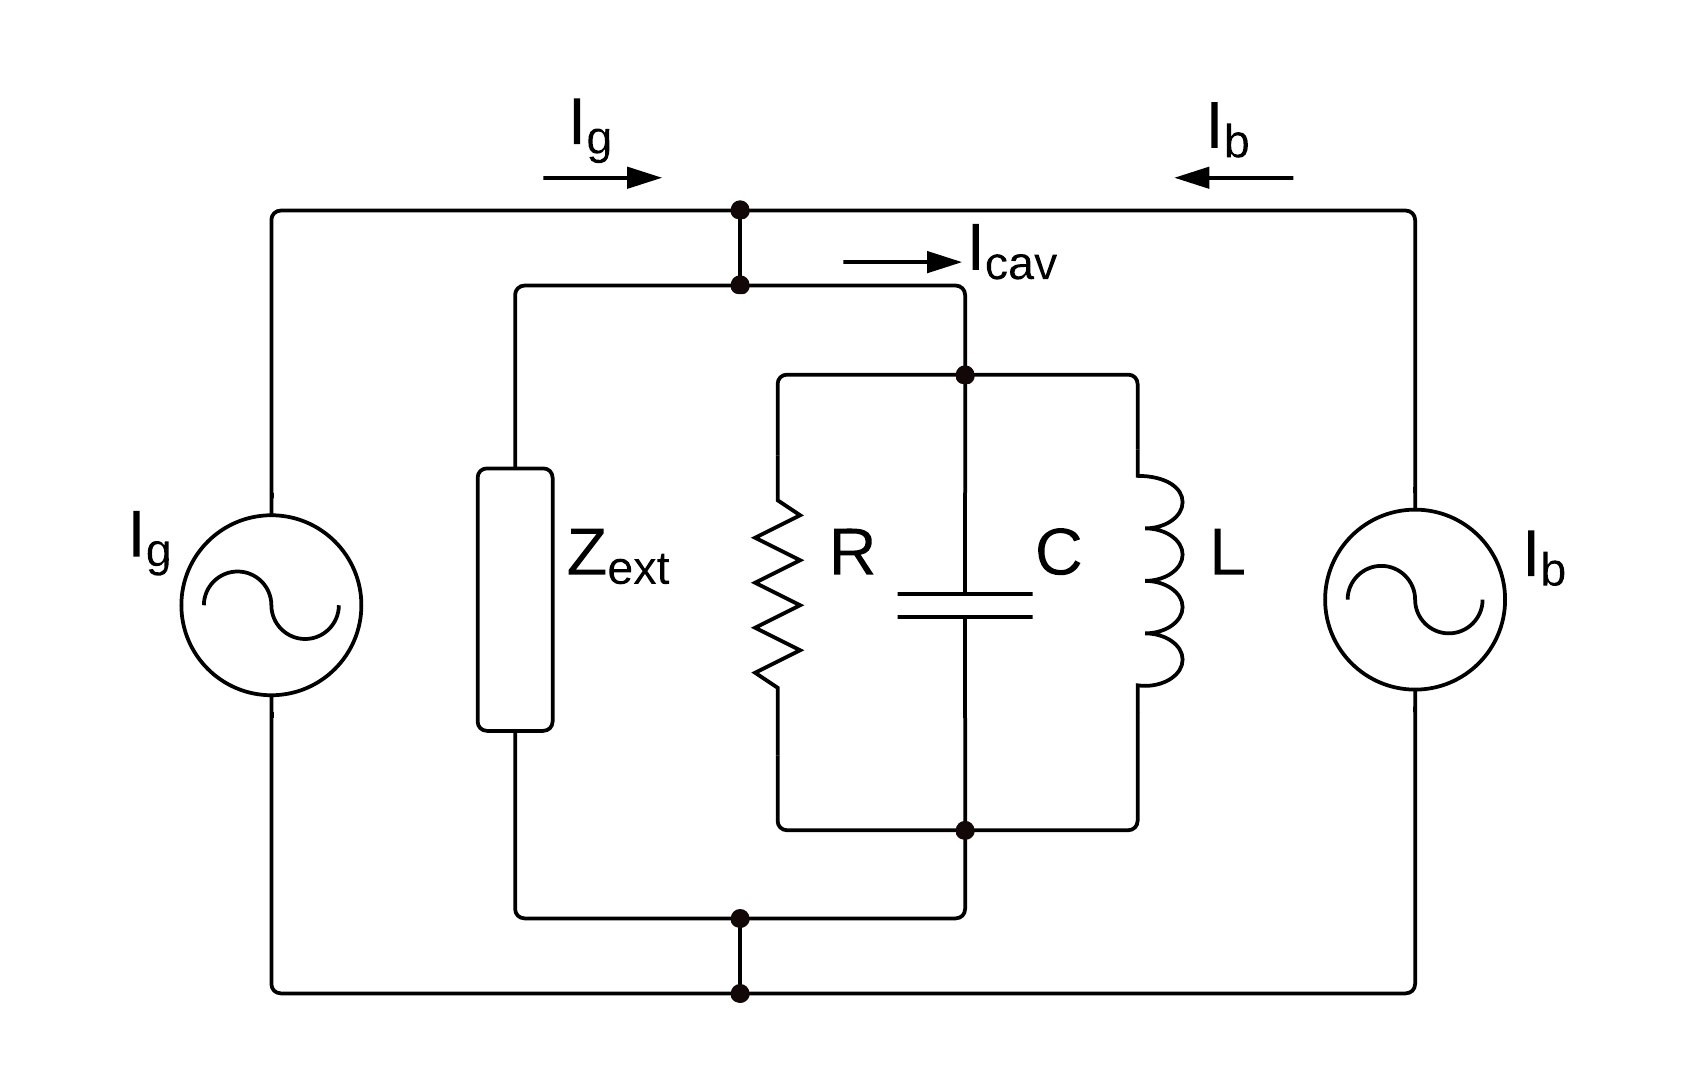
\includegraphics[scale=0.20]{../figures/cavity_eq_circuit.png}
\caption{Electromagnetic eigenmode equivalent circuit.}
\label{fig:cav_eq_circuit}
\end{figure}

A multi-cell cavity is represented by a series of coupled resonators (one per cell in the cavity), each represented by an RLC circuit~\cite{ref:montgomery}. Decomposing the EM cavity fields into eigenmodes and applying the principle of superposition we obtain the representation expressed by equation~\ref{eq:E_probe}~\cite{ref:cell_modes}. The equivalent circuit used to represent one cavity mode is shown in Fig.~\ref{fig:cav_eq_circuit}, where each mode's accelerating voltage is added in order to obtain the cavity overall accelerating voltage, as deduced from Equation~\ref{eq:E_probe}. Each mode has its own value of $\vec V$, $(R/Q)$, $Q_x$, and other characteristics that will be introduced later.

If we apply Kirchhoff's current law to the mode's RLC equivalent circuit (see figure~\ref{fig:cav_eq_circuit}, $\mu$ refers to a particular eigenmode), we get:

\begin{equation}
  \centering \vec I_{\mu} = \vec I_{\rm C_{\mu}} + \vec I_{\rm R_{\mu}} + \vec I_{\rm L_{\mu}}
  \label{eq:currents}
\end{equation}

\noindent where:

\begin{equation}
  \frac{d\vec I_{\rm C_{\mu}}}{dt} = C_{\mu} \cdot \frac{d^2\vec V_{\mu}}{dt^2}\text{,}\qquad \frac{d\vec I_{\rm R_{\mu}}}{dt} = \frac{1}{R_{\rm L_{\mu}}}\frac{d\vec V_{\mu}}{dt} \qquad \text{and}\qquad \frac{d\vec I_{\rm L_{\mu}}}{dt} = \vec V_{\mu}/L_{\mu}
  \label{eq:currents2}
\end{equation}

Differentiating both sides of equation~\ref{eq:currents} and substituting using eq.~\ref{eq:currents2}, the full vector (complex) differential equation for the cavity accelerating voltage $\vec V_{\mu}$ can be written as:

\begin{equation}
  \frac{d^2\vec V_{\mu}}{dt^2} + \frac{1}{R_{\rm L_{\mu}}C_{\mu}}\frac{d\vec V_{\mu}}{dt} + \frac{1}{L_{\mu}C_{\mu}}\vec V_{\mu} = \frac{1}{C_{\mu}}\frac{d\vec I_{\mu}}{dt}
\end{equation}

\noindent which can be expressed as a function of the mode's nominal resonance frequency $\omega_{0_{\mu}}$ ($1/L_{\mu}C_{\mu}=\omega_{0_{\mu}}^2$) and loaded Q ($1/R_{\rm L_{\mu}}C_{\mu}=\omega_{0_{\mu}}/Q_{\rm L_{\mu}}$):
 
\begin{equation}
  \frac{d^2\vec V_{\mu}}{dt^2} + \frac{\omega_{0_{\mu}}}{Q_{\rm L_{\mu}}}\frac{d\vec V_{\mu}}{dt} + \omega_{0_{\mu}}^2 \vec V_{\mu} = \frac{\omega_{0_{\mu}}^2 R_{\rm L_{\mu}}}{Q_{\rm L_{\mu}}}\frac{d\vec I_{\mu}}{dt}
  \label{eq:2nd_order}
\end{equation}

Taking the slowly varying envelope approximation~\cite{ref:svea} ($\omega_{f_{\mu}} \ll \omega_{0_{\mu}}$), separating voltage and current into real and imaginary parts, assuming that the detune frequency varies slowly with respect to the carrier frequency ($\omega_{d_{\mu}} \ll \omega_{0_{\mu}}$) and that $Q_{\rm L_{\mu}} \gg 1$, we can reduce the order of equation~\ref{eq:2nd_order} (a second-order band-pass filter centered at the resonance frequency) to a first-order low-pass filter at baseband~\cite{ref:schilcher}:

\begin{equation}
  \left(1-j\frac{\omega_{d_{\mu}}}{\omega_{f_{\mu}}}\right)\vec V_{\mu} + \frac{1}{\omega_{f_{\mu}}}\frac{d\vec V_{\mu}}{dt} = R_{\rm L_{\mu}} \vec I_{\mu}
  \label{eq:1st_order1}
\end{equation}

\noindent where $\omega_{f_{\mu}}=\omega_{0_{\mu}}/2Q_{L_{\mu}}$ is the mode's bandwidth and $\omega_{d_{\mu}}=2\pi\Delta f_{\mu}$ is the (time varying) detune frequency, given as $\omega_{d_{\mu}}=\omega_{0_{\mu}}-\omega_{ref}$, {\it i.e.}, the difference between actual eigenmode frequency $\omega_{0_{\mu}}$ and the accelerator's time base $\omega_{\rm ref}$.

Transposing the cavity drive term into a combination of the RF source incident wave and beam loading (opposite sign indicating energy absorption by the beam), we can express eq.~\ref{eq:1st_order1} as:

\begin{equation}
  \left(1-j\frac{\omega_{d_{\mu}}}{\omega_{f_{\mu}}}\right)\vec V_{\mu} + {\frac{1}{\omega_{f_{\mu}}}}\frac{d\vec V_{\mu}}{dt} =  2\vec K_{\rm g}\sqrt{R_{\rm g_{\mu}}} - R_{\rm b_{\mu}}\vec I_{\rm beam}
  \label{eq:1st_order2}
\end{equation}

\noindent where $\vec K_{\rm g}$ is the incident wave amplitude in $\sqrt{\rm Watts}$, $R_{\rm g_{\mu}}=Q_{\rm g_{\mu}}(R/Q)_{\mu}$ is the coupling impedance of the drive port, $\vec I_{\rm beam}$ is the beam current, and $R_{\rm b_{\mu}}=Q_{\rm L_{\mu}}(R/Q)_{\mu}$ is the coupling impedance to the beam.

The overall $Q_{\rm L_{\mu}}$ is given as $1/Q_{\rm L_{\mu}}=1/Q_{0_{\mu}}+1/Q_{g_{\mu}}+1/Q_{p_{\mu}}$, where $1/Q_{0_{\mu}}$ represents losses to the cavity walls, $1/Q_{g_{\mu}}$ represents coupling to the input coupler, and $1/Q_{p_{\mu}}$ represents coupling to the field probe. $(R/Q)_{\mu}$ is the shunt impedance of the mode in Ohms, a pure geometry term computable for each particular eigenmode using E\&M codes like Superfish. Physically, shunt impedance relates a mode's stored energy $U_{\mu}$ to the accelerating voltage it produces, according to 

\begin{equation}
  U_{\mu} = \frac{V_{\mu}^2}{(R/Q)_{\mu}\omega_{0_{\mu}}}
\end{equation}

The only assumptions in the above formulation are that the cavity losses are purely resistive, and thus expressible with a fixed $Q_{0_{\mu}}$, and that no power is launched into the cavity from the field probe.  If other ports have incoming power, there would be additional terms of the same form as $2\vec K_g\sqrt{R_g}$.

The $\frac{\omega_{d_\mu}}{\omega_{f}}$ term in \ref{eq:1st_order2} (the imaginary component of the cavity pole at baseband) represents detuning. In software or hardware implementations, we can alternatively modulate that term with Lorentz perturbations, or use a purely real pole ($\omega_f$) and modulate the frequency of the drive term. We prefer the latter, more convinient in computational terms. We then define a vector $\vec{S}_{\mu}$ such that:

\begin{equation}
\vec{V}_{\mu} = \vec{S}_{\mu}e^{j\theta_{\mu}}
\label{eq:V_mu}
\end{equation}

\begin{equation}
\frac{d\theta_{\mu}}{dt} = \omega_{d_\mu}
\label{eq: d0_dt}
\end{equation}

\noindent yielding:

\begin{equation}
\left(1 - j\frac{\omega_{d_\mu}}{\omega_{f_{\mu}}}\right)\vec{S}_{\mu}e^{j\theta_{\mu}} + \frac{1}{\omega_{f_{\mu}}}
    \left(\frac{d\vec{S}_{\mu}}{dt}e^{j\theta_{\mu}} + \vec{S}_{\mu} \cdot j\omega_{d_{\mu}}e^{j\theta_{\mu}}\right) = 2\vec{K}_{g}\sqrt{R_{g_{\mu}}} - R_{b_{\mu}}\vec{I}_{\rm beam}
\label{eq Gov_S}
\end{equation}

\noindent The governing equation for the mode's accelerating voltage can thus be written as a set of two first order differential equations (eqs.~\ref{eq: dS_dt} and~\ref{eq: d0_dt}):

\begin{equation}
  \frac{d\vec{S}_{\mu}}{dt} = -\omega_{f_{\mu}}\vec{S}_{\mu} + \omega_{f_{\mu}}e^{-j\theta_{\mu}}\left(2\vec{K}_g\sqrt{R_{g_{\mu}}} 
    - R_{b_{\mu}}\vec{I}_{\rm beam} \right)
\label{eq: dS_dt}
\end{equation}

Note that this state-variable equation is a pure low-pass filter, an advantage especially in the FPGA implementation.

\subsection{Software implementation}

\begin{figure}
\centering
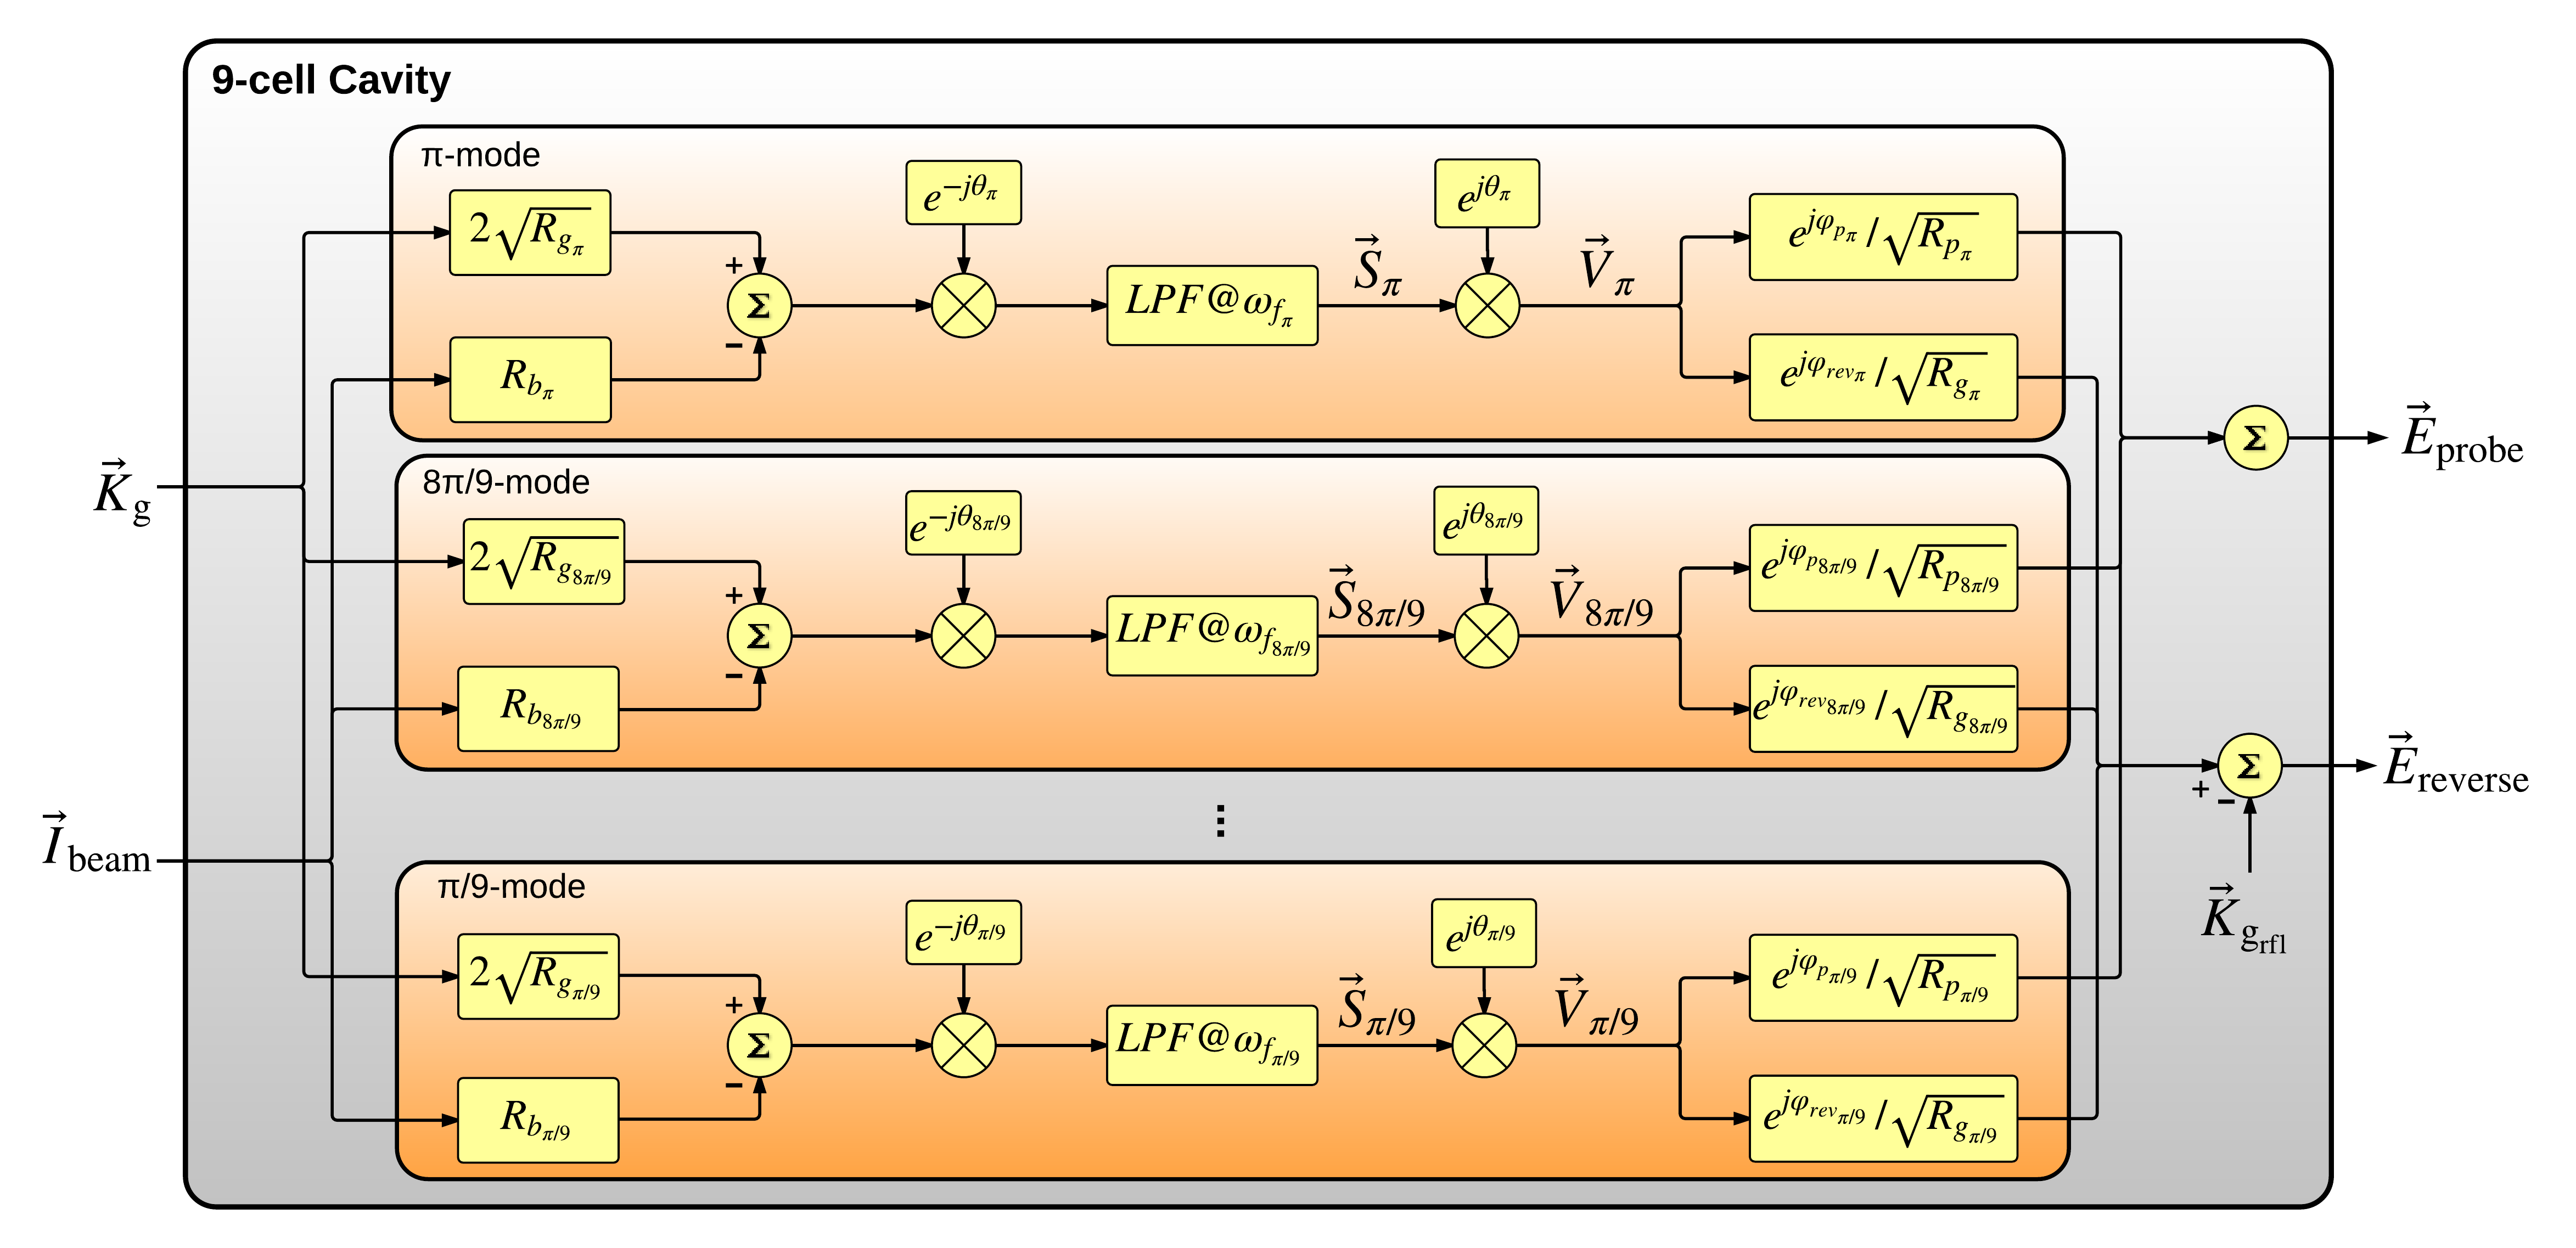
\includegraphics[scale=0.4]{../figures/Cavity_modes.png}
\caption{Data path for the computation of a 9-cell cavity model.}
\label{fig:RF_cavity_block_diagram}
\end{figure}

We started this section with the definition of $\vec E_{\rm probe}$ and $\vec E_{\rm reverse}$ given by equations \ref{eq:E_probe} and \ref{eq:E_reverse} respectively. These equations express the measured probe and reverse fields as a function of eigenmode voltages ($\vec V_\mu$) and their respective port couplings. We also defined the state-variable equation governing the accelerating voltage for each eigenmode in Equation~\ref{eq: dS_dt}, where $\vec{V}_{\mu} = \vec{S}_{\mu}e^{j\theta_{\mu}}$. We can therefore compute the cavity probe and reverse signals as a function of the incident wave $\vec K_{\rm g}$ and the beam current $\vec I_{\rm beam}$.

Figure~\ref{fig:RF_cavity_block_diagram} shows the data path implemented in software in order to compute the response of a nine-cell cavity (which can be configured for any type of cavity given the definition of the electrical eigenmodes and couplings). Each internal bock represents the implementation of Eq.~\ref{eq: dS_dt} for each eigenmode, and the summing junction at the end (taking the pre-factored eigenmode voltages) represents the computation of $\vec E_{\rm probe}$ and $\vec E_{\rm reverse}$ using Equations \ref{eq:E_probe} and \ref{eq:E_reverse}.

Note that there are two aspects represented in Fig.~\ref{fig:RF_cavity_block_diagram} which are not shown in the equations. The first one is the use of $\vec K_{\rm g_{rfl}}$ instead of $\vec K_{\rm g}$, as well as the terms $e^{j\varphi_{x}}$ in the factoring of each $\vec V_\mu$ term before the summing junctions. These terms represent frequency dependent propagation through cables and waveguides. In the case of the incident wave, if we define $TF_{\rm wg}(s)$ as the transfer function in Laplace domain of a wide-band filter representing the waveguide between the directional coupler on the high-power forward path and the cavity, we get:

\begin{equation}
 \vec K_{\rm g_{rfl}}(s) = \vec K_{\rm g}(s) \cdot TF_{\rm wg}(s)
\end{equation}

\noindent where the minus sign of the reflection on the cavity coupler is represented in the summing junction. This transformation takes into account the propagation of the reflection of the incident wave back to the directional coupler.
The cavity probe and reverse path also follow a similar transformation but in this case represented by a phase shift through the coaxial cable from the cavity probe and reverse ports and their respective ADCs in the LLRF. These phase shifts are represented by the $e^{j\varphi_{\rm rev_{\mu}}}$ and $e^{j\varphi_{\rm p_{\mu}}}$ terms in Fig.~\ref{fig:RF_cavity_block_diagram}, which are frequency dependent due to dispersion in the coaxial cables, and therefore need to be applied at this stage of the computation (before the summing junction).

The second aspect which has not been covered yet is the numerical discretization of the first-order low-pass filter in the cavity response, represented by the blocks labeled $LPF@\omega_{f_{\mu}}$ in Fig.~\ref{fig:RF_cavity_block_diagram}. The ODE integration is derived in Appendix~\ref{App:ODE_integration}, where Equation~\ref{eq: dS_dt} can be written as Equation~\ref{eq:exp_diff2}, where

\begin{equation}
 \vec V_{\rm out} = \vec S_{\mu} \mbox{ , } p = -\omega_f \mbox{ and, } \vec V_{\rm in} = e^{-j\theta_{\mu}} \left(2\vec{K}_g\sqrt{R_{g_{\mu}}} - R_{b_{\mu}}\vec{I}_{\rm beam}\right)
\end{equation}

\noindent as it can be deduced from Fig.~\ref{fig:RF_cavity_block_diagram}. This block solves for $\vec S_{\mu}$, which is translated to the mode's accelerating voltage using equations~\ref{eq:V_mu} and~\ref{eq: d0_dt}, as indicated in the block diagram.

In summary, using the computations shown in Figure~\ref{fig:RF_cavity_block_diagram} (couplings, rotations, etc.) combined with the numerical discretization of the cavity filter described in Appendix~\ref{App:ODE_integration} applied every discrete simulation step, we can obtain time-series simulated data representing signal propagation through the multi-cell RF cavity, including the different eigenmodes and dispersion through cables and waveguides.

\subsection{Simulation results}

\begin{figure}
\centering
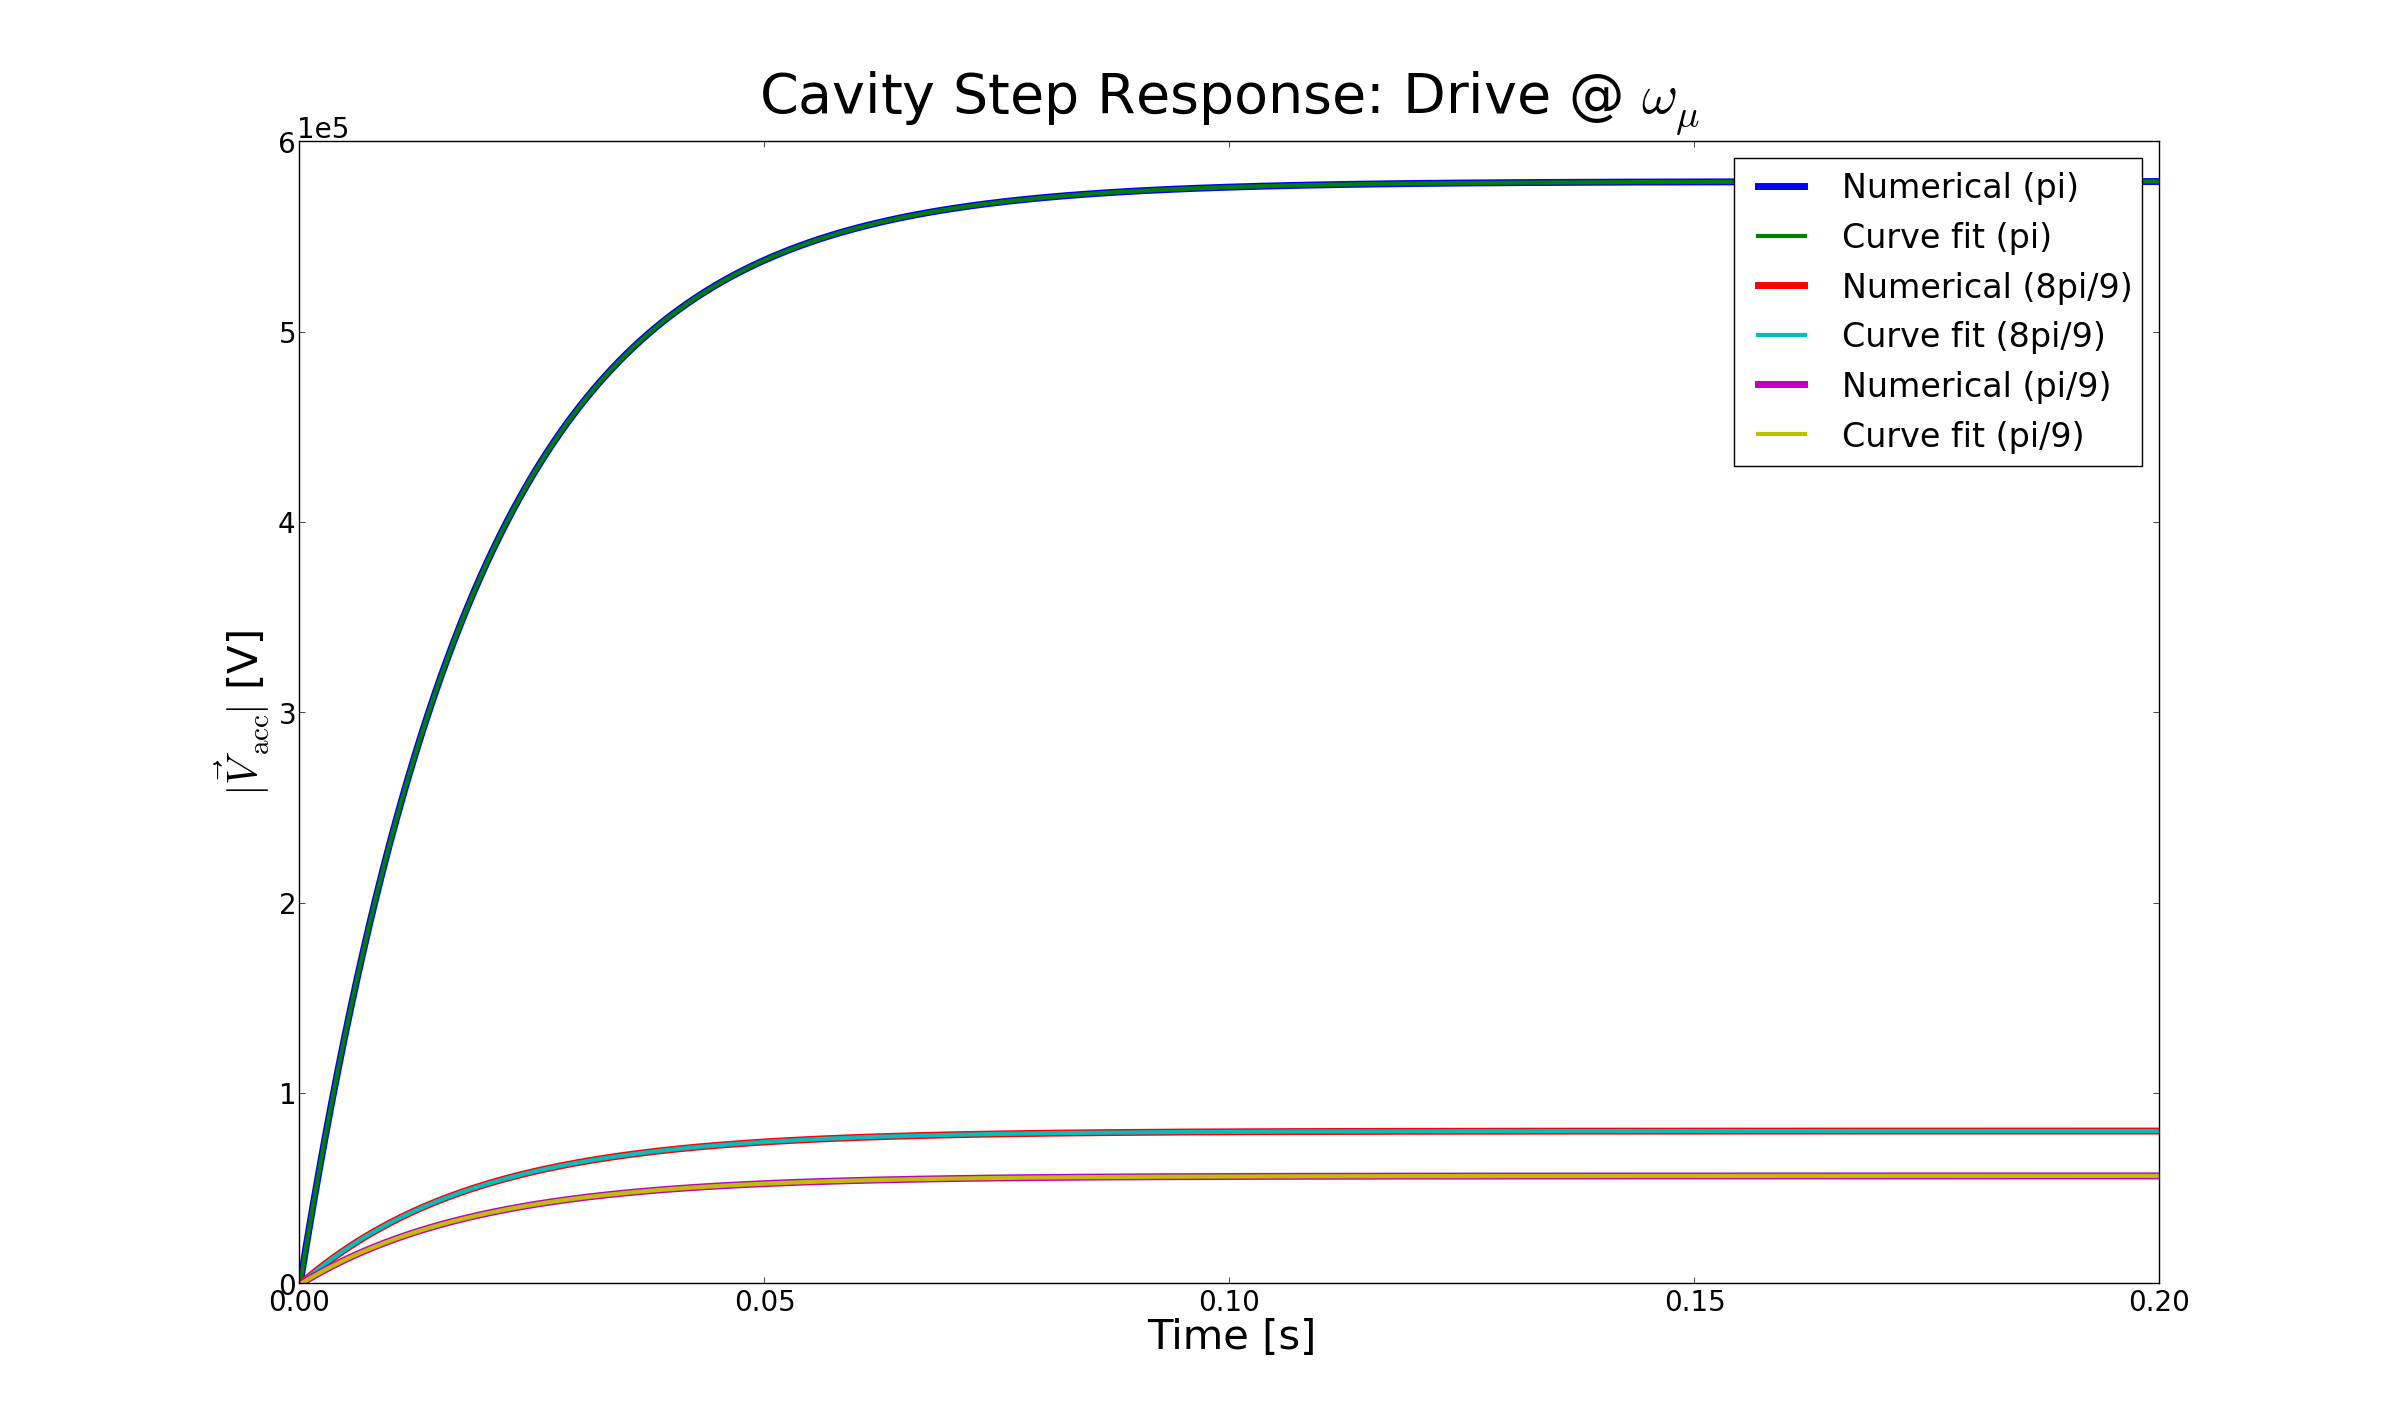
\includegraphics[scale=0.26]{../figures/cavity_test_drive.png}
\caption{Cavity unit test: Cavity response to a step function on the RF drive signal, where the input signal is at the each mode's resonance frequency.}
\label{fig:cav_step1}
\end{figure}

A few unit tests have been designed in order to check the correspondence between the numerical simulation results and the theoretical equations. The unit under test here is the cavity model illustrated in Fig.~\ref{fig:RF_cavity_block_diagram}. Some of these tests have little physical meaning and are even unrealizable in practice, however this is the beauty of the simulation world, where one can isolate effects in the calculations for different purposes, in this case in order to verify its own proper operation.

Figures~\ref{fig:cav_step1} and~\ref{fig:cav_step2} show the step response of three individual eigenmodes ($\pi$, $8\pi/9$ and $\pi/9$ modes in this case). In these tests, the cavity routine is configured to have one individual mode and the time-series simulation is run three times to obtain each one of the three curves on the plots. This allows us to fit the step response curves for each eigenmode individually, thus deducing mode bandwidths and couplings from the curve fit results. Both the numerical curves and the curve fits are shown for each simulation run, where (in the absence of noise as in this case) there is a very good correspondance between the two (in the order of $10^{-5}$ RMS errors).

\begin{figure}
\centering
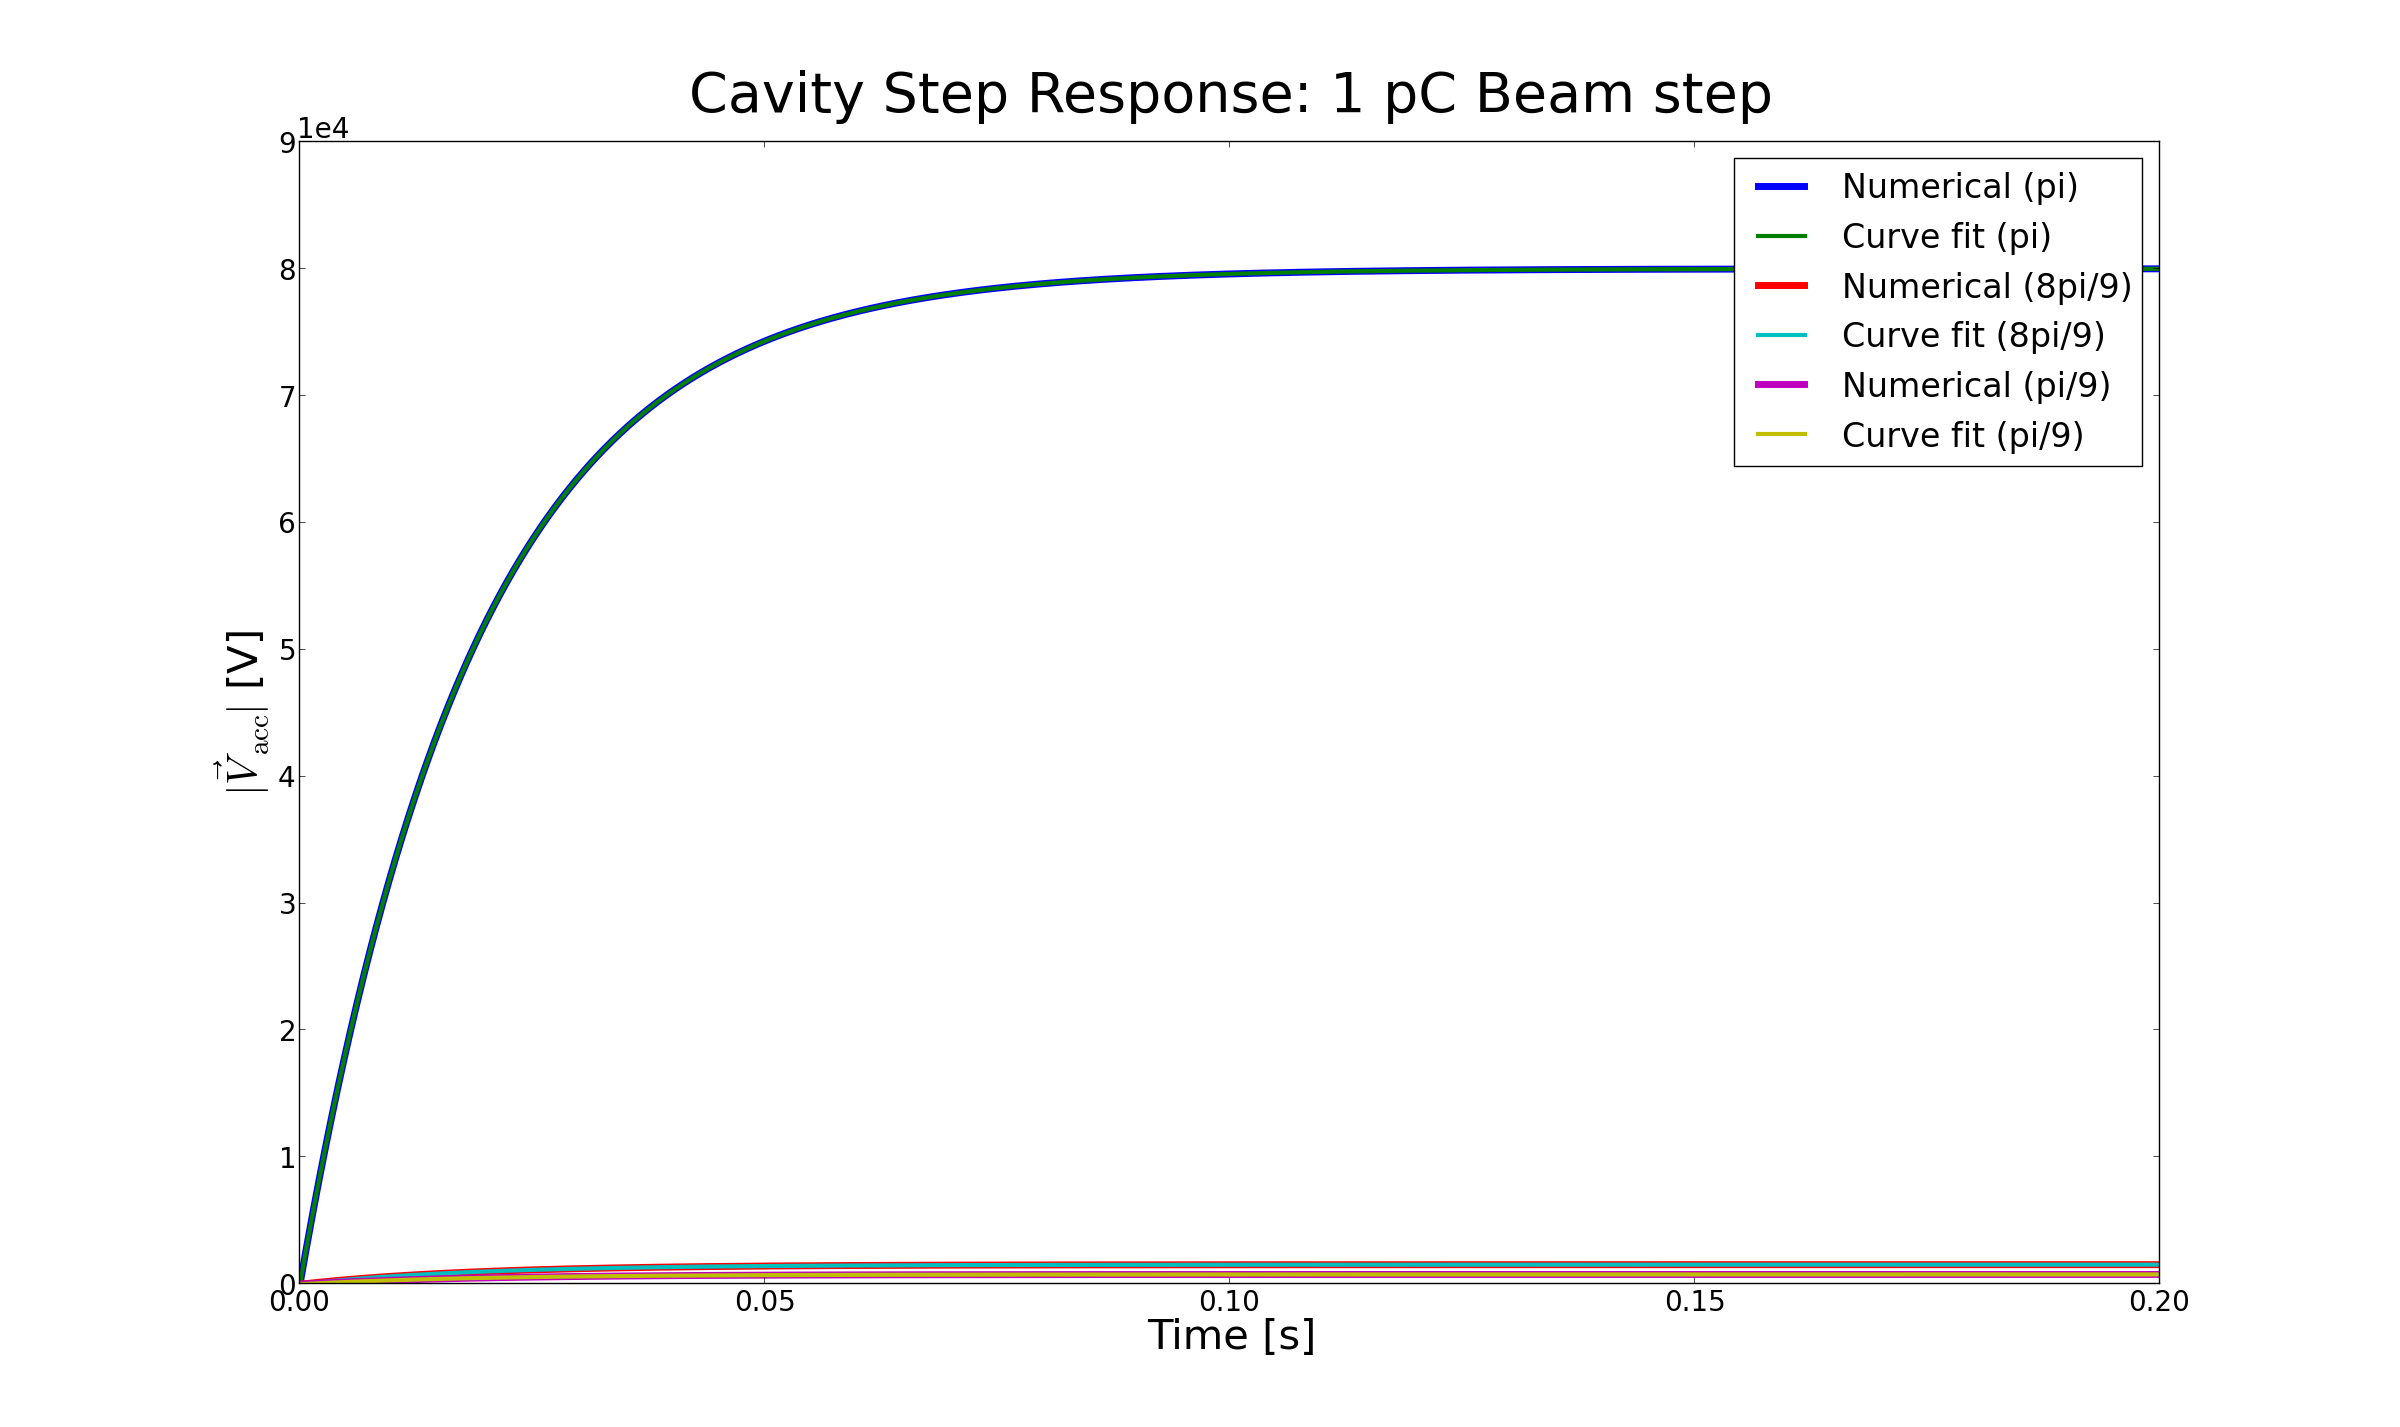
\includegraphics[scale=0.26]{../figures/cavity_test_beam.png}
\caption{Cavity unit test: Step response, beam coupling.}
\label{fig:cav_step2}
\end{figure}

In Fig.~\ref{fig:cav_step1} we introduce a unit amplitude step signal on the RF drive port at the mode's resonance frequency ($\omega_{0_{\mu}}$), which is equivalent to driving the input drive signal with a vector of unity length rotating at the mode's detune frequency ($\omega_{f_{\mu}}$). The input signals are then: $\vec K_{\rm g}=e^{j\theta_{\mu}}$ ($d\theta_{\mu}/dt = \omega_{d_\mu}$) and $\vec I_{\rm beam}=0$. As a result no ringing is observed. The model is designed to have unity gain at the mode's center frequency and one can therefore deduce couplings to the drive input by measuring the steady-state values. The step response is then fit to a 1st-order differential equation and the bandwidth of each mode is deduced, matching the configuration settings. This test provides a verification for the incident wave coupling impedance ($R_{\rm g_{\mu}}$ in eq.~\ref{eq: dS_dt}) as well as the mode's bandwidth ($\omega_{f_{\mu}}$ in the same equation).

In Fig.~\ref{fig:cav_step2} we introduce a step signal on the beam input signal equivalent to 1 pC beam charge (this number is just anecdotal since we are interested in measuring couplings, etc.). In this case $\vec K_{\rm g}=0$, providing means to deduce the beam coupling impedance for each eigenmode in a similar manner as described in the previous test. In both tests we also evaluate the probe ($\vec E_{\rm probe}$ in eq.~\ref{eq:E_probe}) and reverse field signals ($\vec E_{\rm reverse}$ in eq.~\ref{eq:E_reverse}) and compare them to the accelerating voltages, therefore being able to deduce the coupling impedances to the probe and drive ports for each eigenmode ($Q_{\rm p_{\mu}}(R/Q)_{\mu}$ and $Q_{g_{\mu}}(R/Q)_\mu$ in eqs.~\ref{eq:E_probe} and~\ref{eq:E_reverse} respectively).

\begin{figure}
\centering
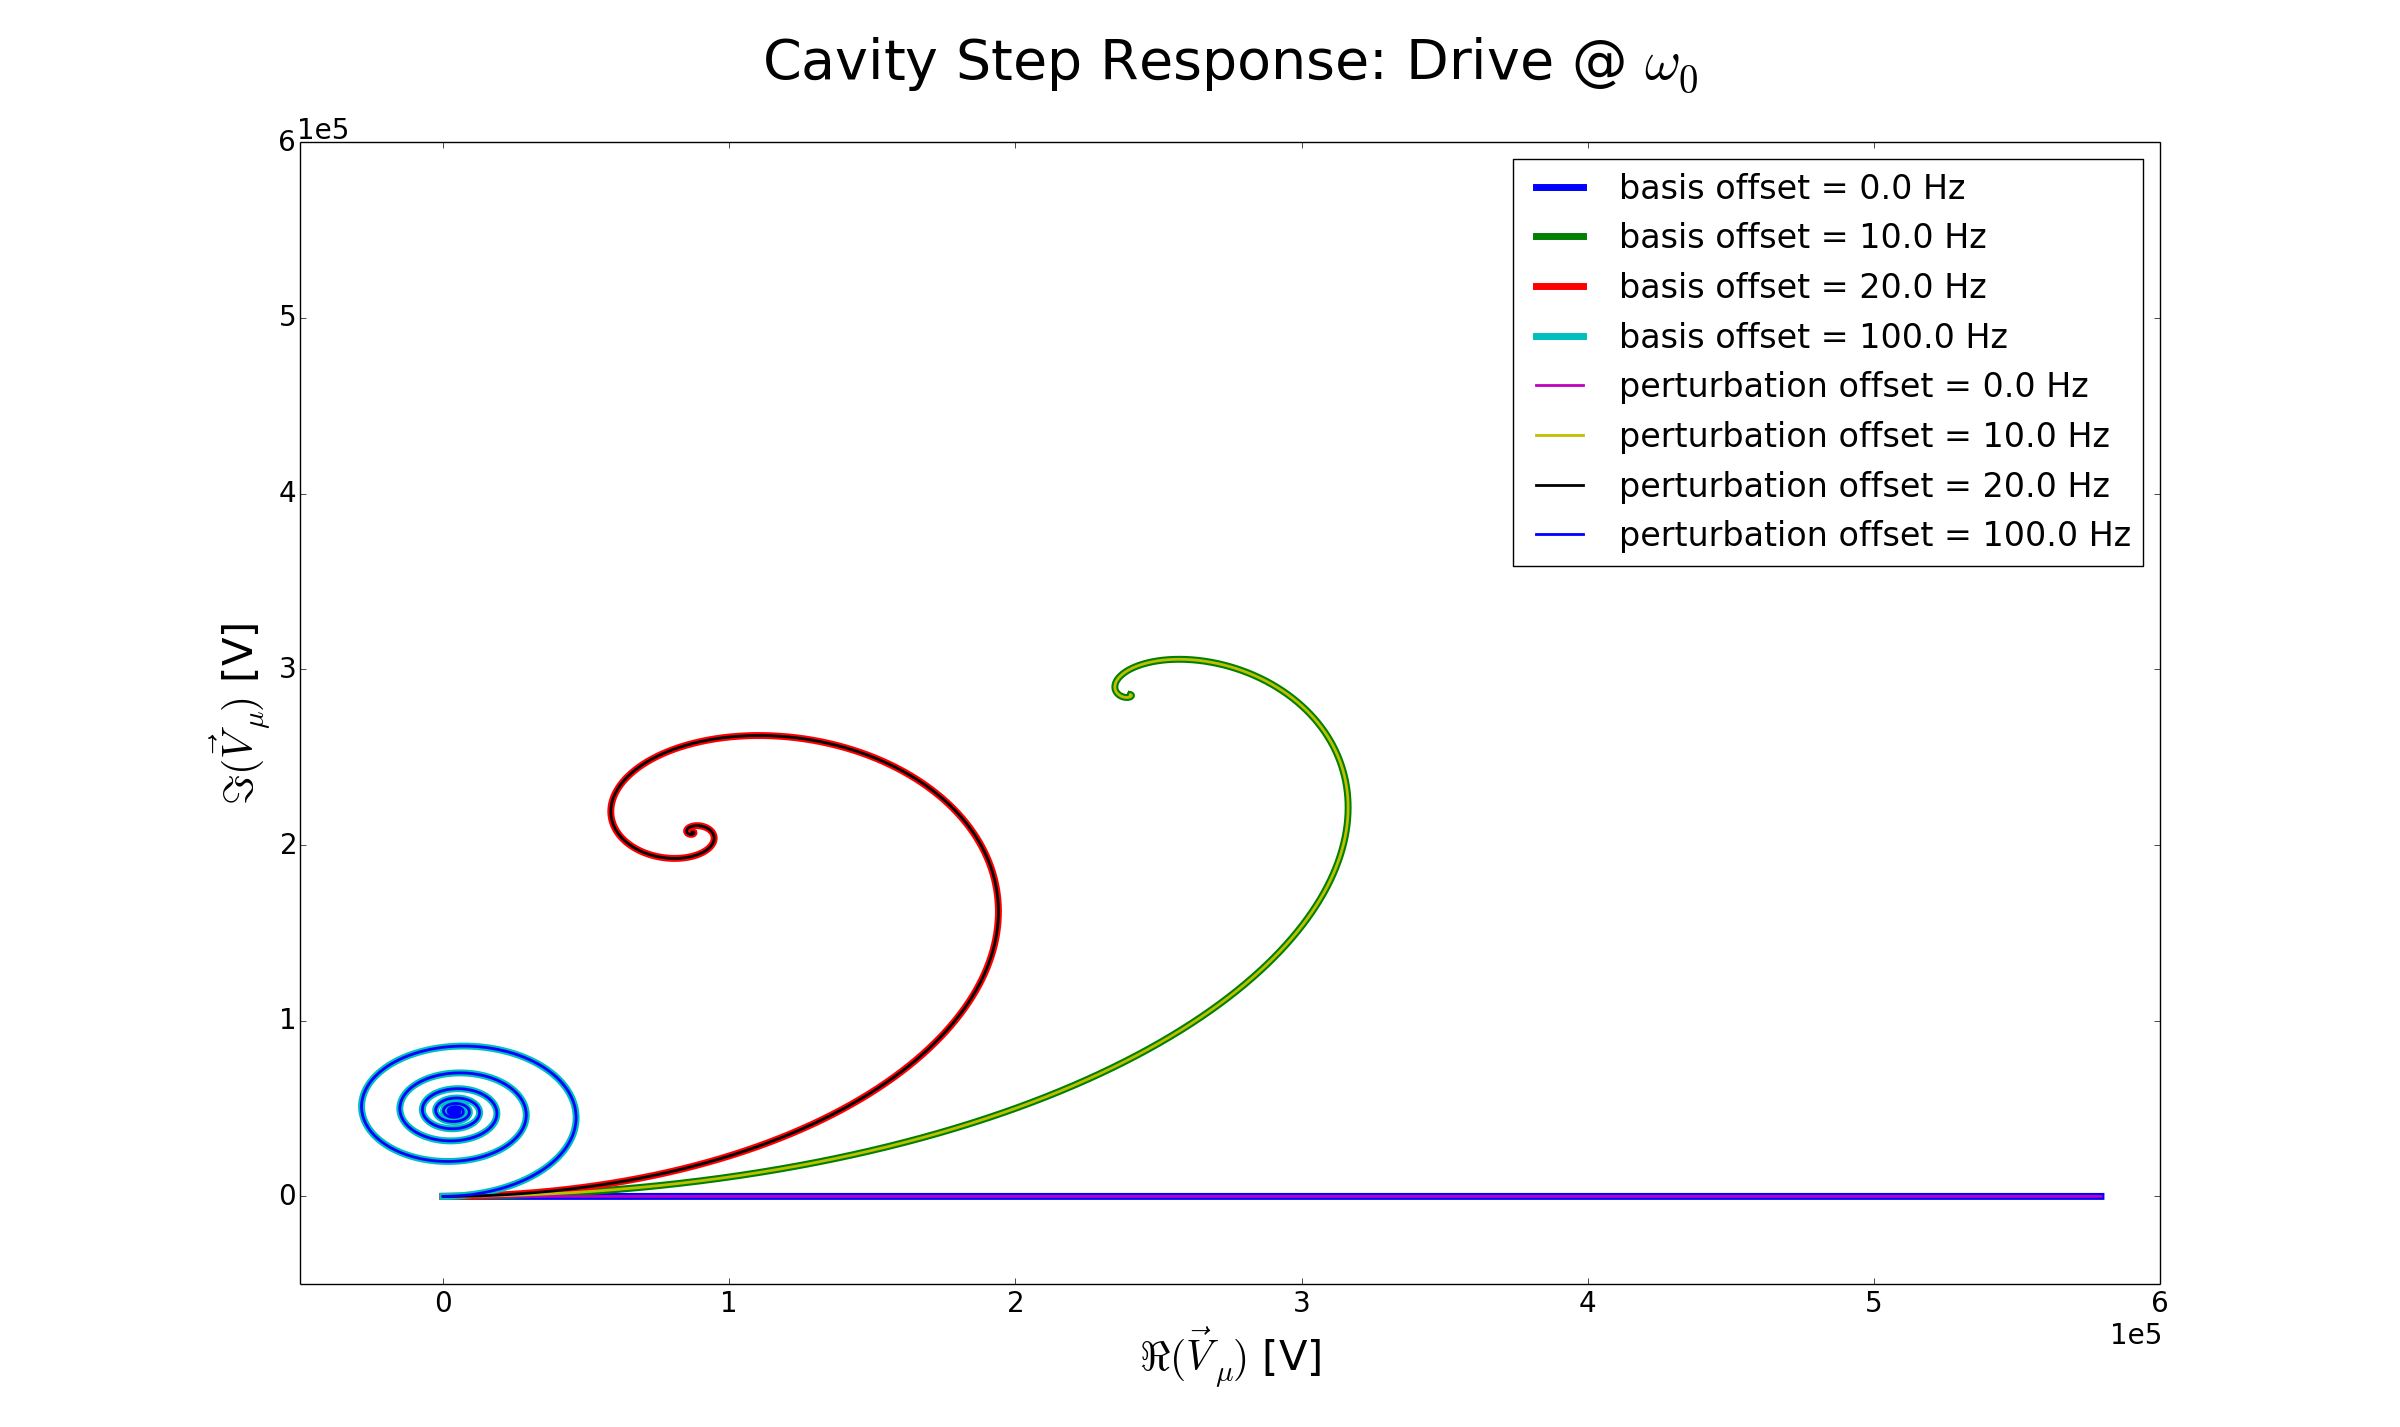
\includegraphics[scale=0.24]{../figures/cavity_test_freqs.png}
\caption{Cavity unit test: Step response RF drive coupling at $\omega_{\rm ref}$ for three different frequency offsets.}
\label{fig:cav_step3}
\end{figure}

At this point we have demonstrated the low-pass filter blocks in Fig.~\ref{fig:RF_cavity_block_diagram} as well as the couplings to the input and output ports. We are now going to demonstrate an important feature (cavity detuning). One can both configure an electrical eigenmode to have a static frequency offset with respect to the RF reference, as well as introducing a time-varying frequency offset due to Lorentz forces or other perturbations.

\begin{figure}
\centering
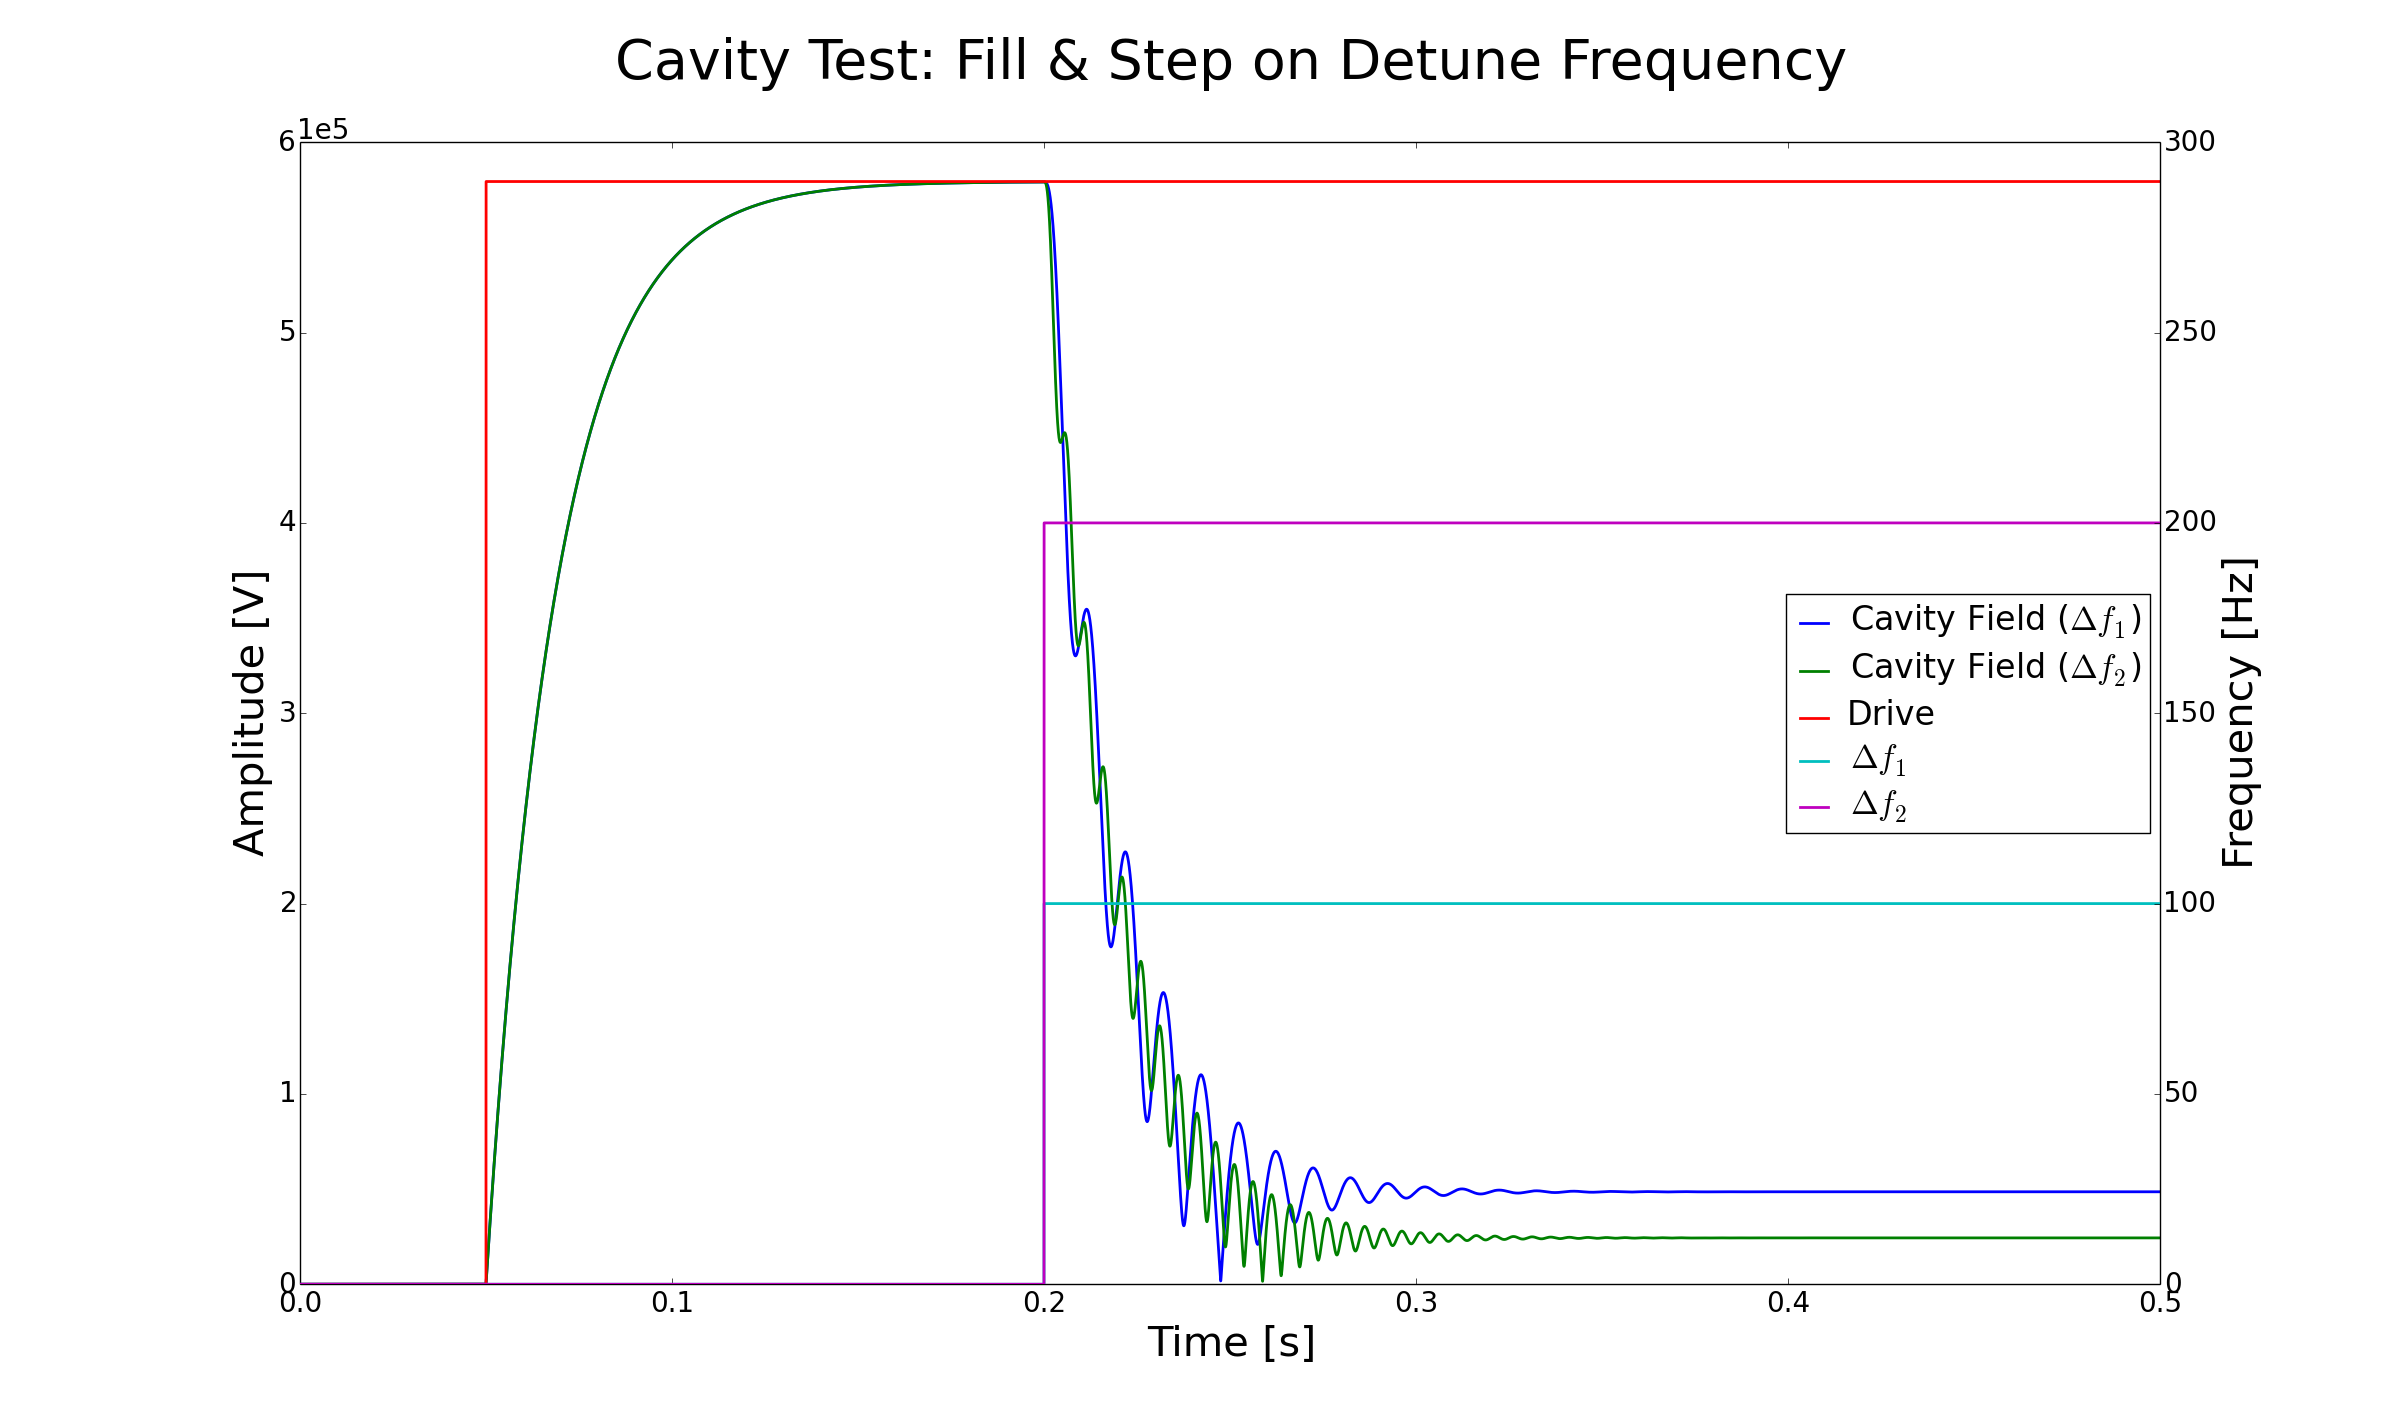
\includegraphics[scale=0.24]{../figures/cavity_test_detune.png}
\caption{Cavity unit test: Step response RF drive coupling at $\omega_{\rm ref}$ and step on the detune frequency (amplitude)}
\label{fig:cav_step4}
\end{figure}

In Fig~\ref{fig:cav_step3} we introduce a unit amplitude step signal on the RF drive port at the RF reference frequency ($\omega_{\rm ref}$) (instead of at each mode's resonance frequency as in the case of Fig.~\ref{fig:cav_step1}). Each curve is reproduced in two equivalent ways in order to exercise two features of the software: first by sweeping the setting for the so-called basis, or static, offset frequency (the frequency offset between the mode's resonance frequency and the RF reference), and second by sweeping the setting for the frequency shift due to perturbations such as Lorentz forces. All curves correspond to the same mode's accelerating voltage, where only the frequency offset changes, and is plotted in the complex plane to observe the different degrees of ringing as frequency offsets are introduced.

\begin{figure}
\centering
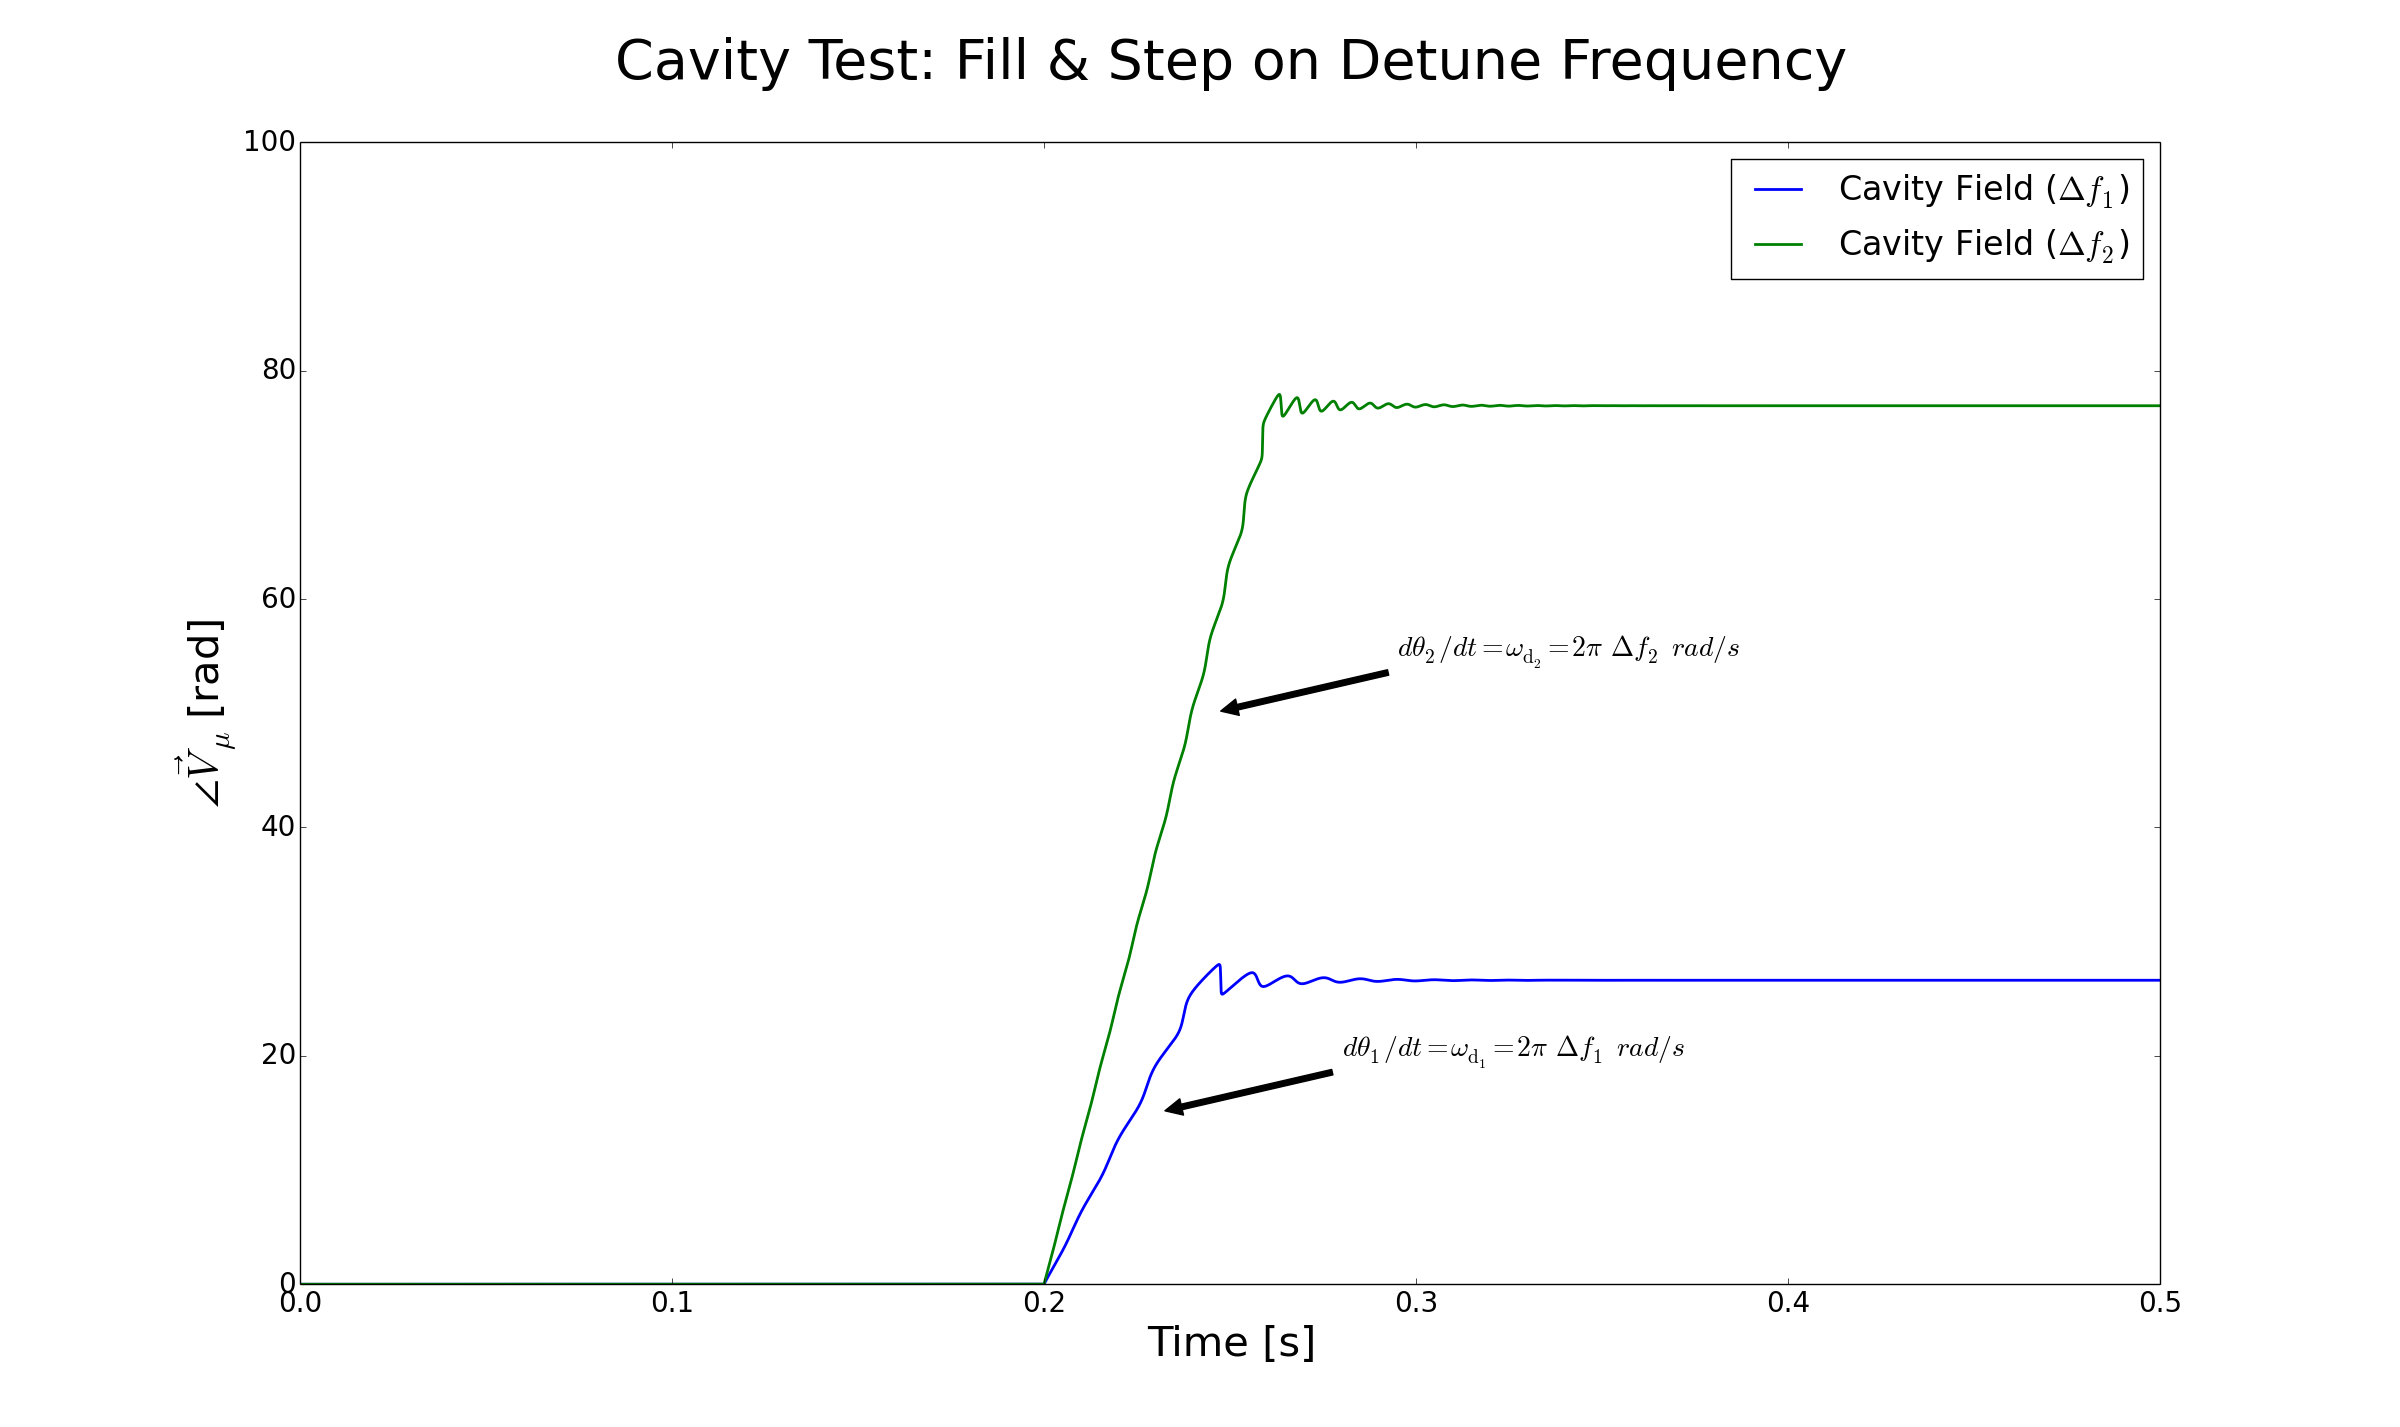
\includegraphics[scale=0.26]{../figures/cavity_test_detune_phase.png}
\caption{Cavity unit test: Step response RF drive coupling at $\omega_{\rm ref}$ and step on the detune frequency (phase).}
\label{fig:cav_step5}
\end{figure}

Fig.~\ref{fig:cav_step4} shows a combination of the previous exercises, where the cavity mode is initially in perfect resonance. A step is applied to the drive signal at the mode's resonance frequency and the cavity field fills up following its time constant (quantified in previous tests). Then, we apply a step to the detune frequency of 10 to 20 times the bandwidth of the cavity mode and we observe the cavity decay following its time constant along with ringing induced by the cavity being out of tune. Note that the frequency modulations of the cavity field correspond to the frequency offset applied in each case, and for the case where the step applied is of 100 Hz, the steady-state value is equivalent to the one observed in fig.~\ref{fig:cav_step3} for the same value of freqency offset.


The frequency modulation can be better observed in Fig.~\ref{fig:cav_step5}, where the phase of the two cavity field signals is shown. Note the 0 deg. phase during fill time when the cavity is perfectly in tune (and RF drive is purely real). The phase then starts varying when the frequency offset step is applied. The slope of the phase corresponding to the angular frequency shift applied, as indicated in the figure.

\newpage

\begin{appendix}

\section{Appendix}

\subsection{ODE Integration of single-pole low-pass filter}
\label{App:ODE_integration}

\begin{figure}
\centering
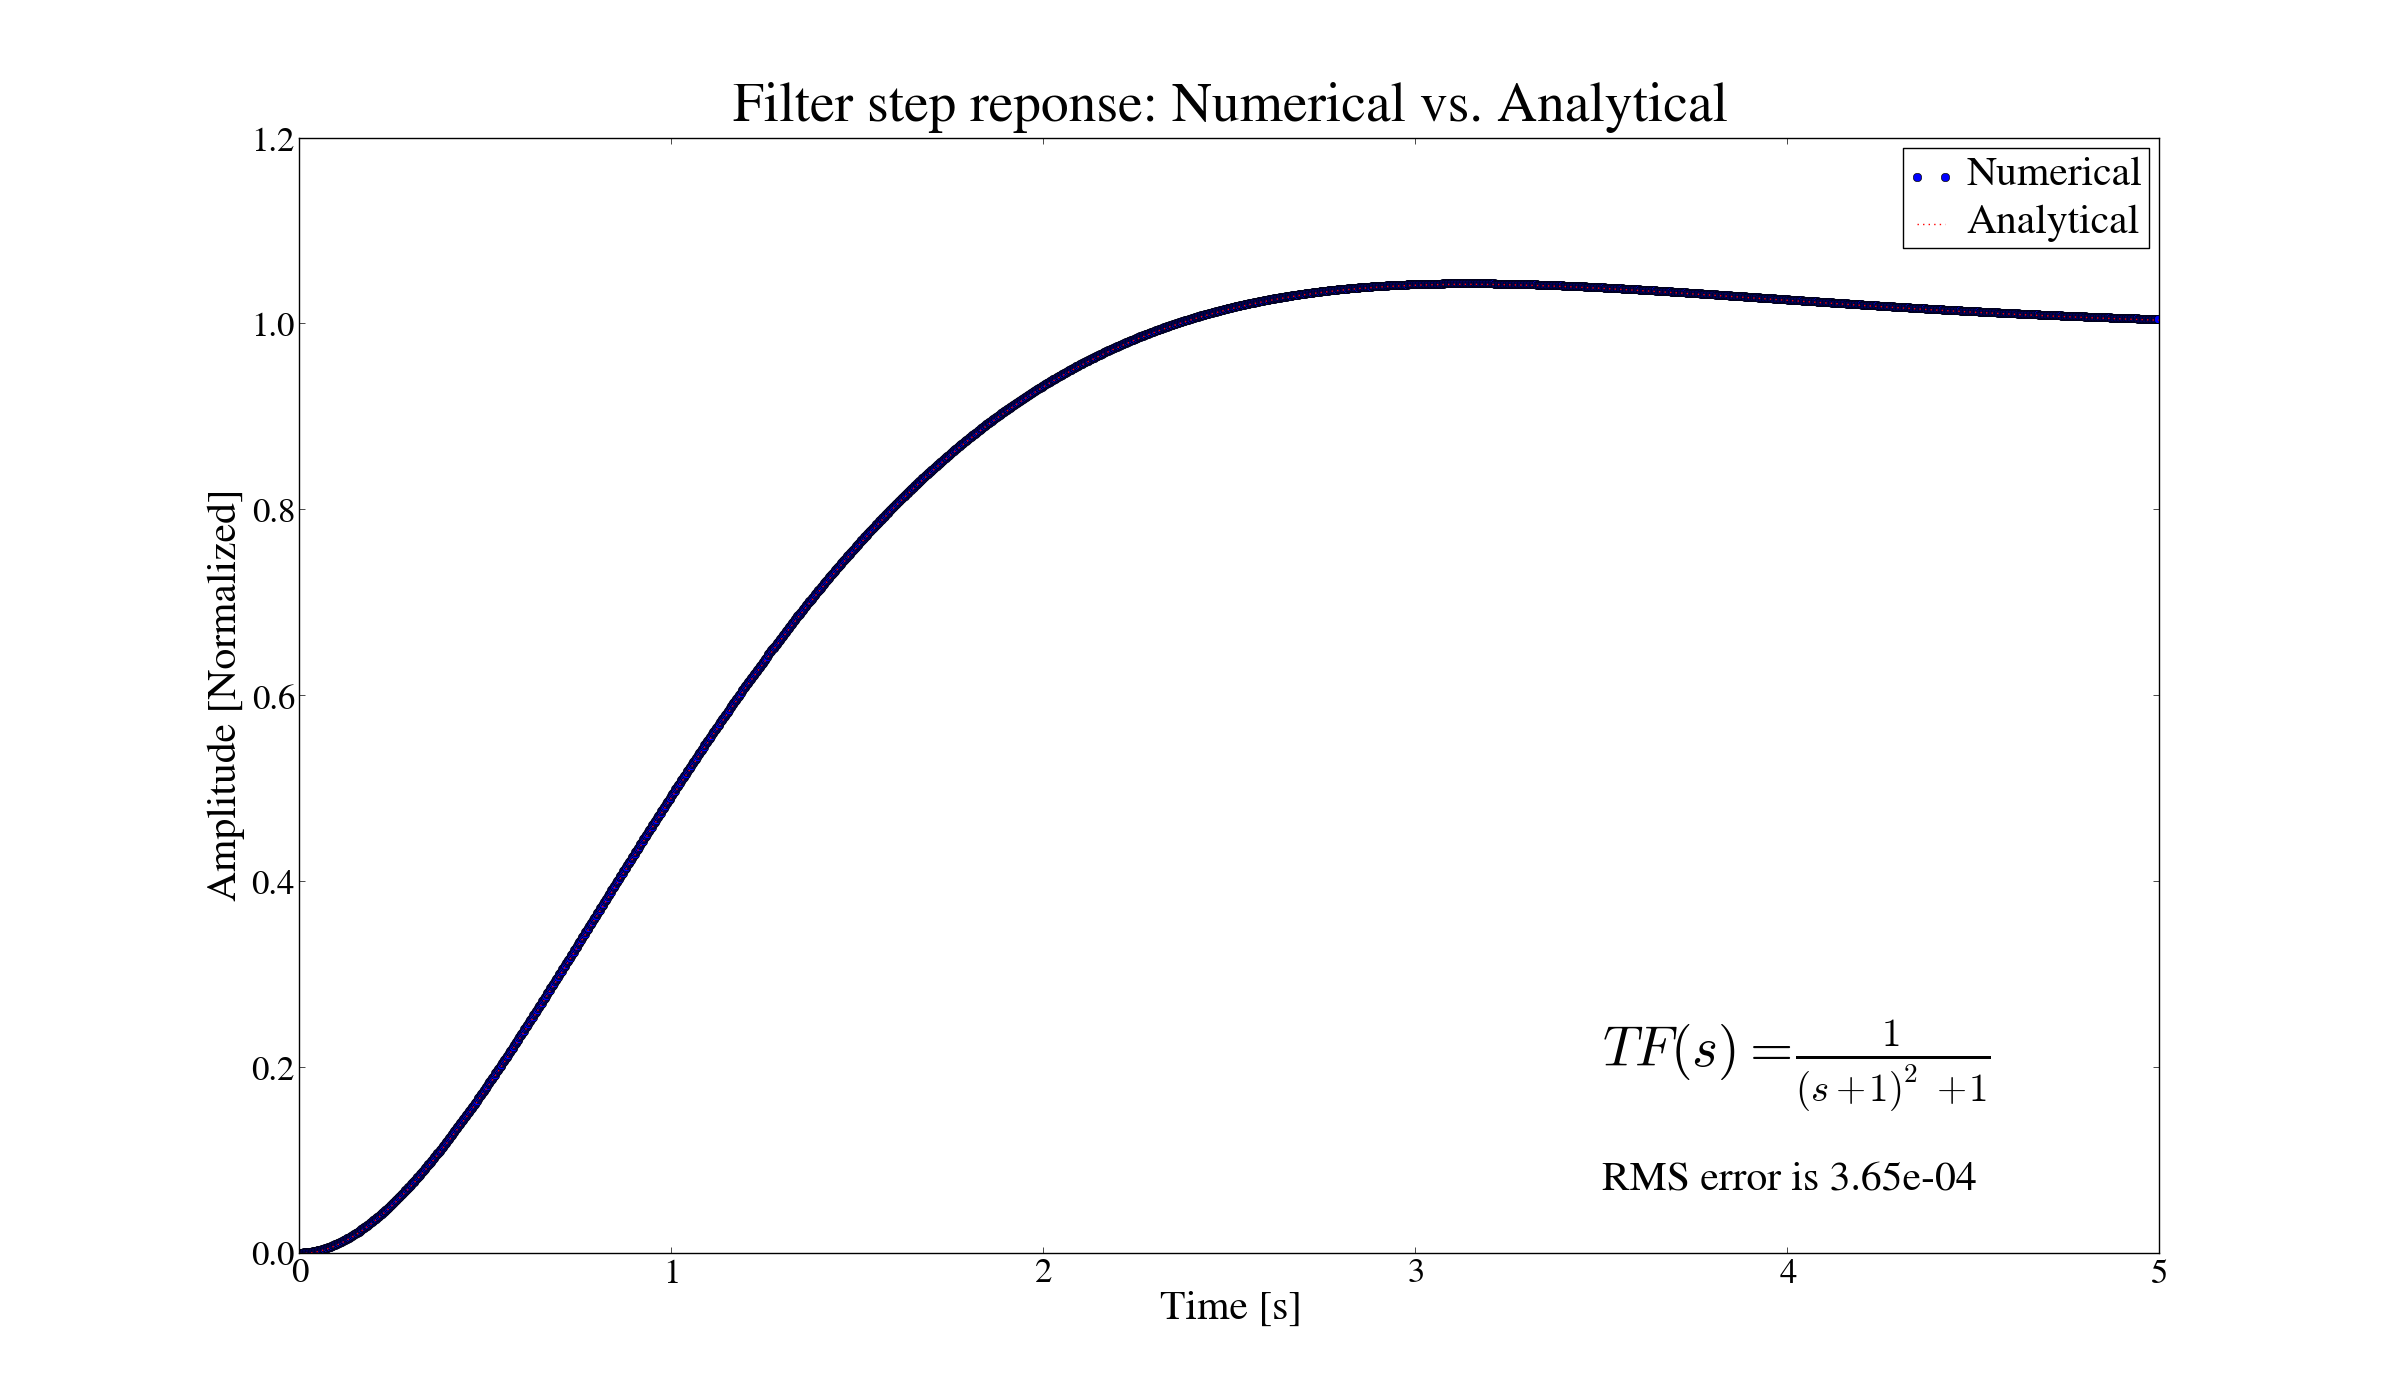
\includegraphics[scale=0.265]{../figures/filter_step_response.png}
\caption{Comparison between numerical and analytical filter step response.}
\label{fig:filter_step_response}
\end{figure}

Start with the first order differential equation for a single-pole low pass filter. Its transfer function is expressed in Laplace form as

\begin{equation}
 TF(s)=\frac{\vec V_{\rm out}(s)}{\vec V_{\rm in}(s)} = \frac{1}{s-p}
\end{equation}

\noindent where $\vec V_{\rm in}$ and $\vec V_{\rm out}$ are the input and output signals, and $p$ is the pole location. Make the differentiation explicit, and rearrange to get a form consistent with state-variable numerical ODE integration,

\begin{equation}
 \frac{d\vec V_{\rm out}(t)}{dt} = \vec V_{\rm in}(t) + p\cdot \vec V_{\rm out}(t)
\label{eq:exp_diff}
\end{equation}

The simplest expression for a 'next' value at step $n$ in a discrete time \emph{ansatz} is

\begin{equation}
 \vec V_{\rm out}^n = \left( 1 + \Delta t \cdot p\right) \vec V_{\rm out}^{n-1} + \Delta t \cdot V_{\rm in}^n
\end{equation}

\noindent To improve convergence properties in the case where $\Delta t \cdot p$ is not tiny, approximate the trajectory of $\vec V_{\rm in}$ and $\vec V_{\rm out}$ as linear within a single time step. Specifically, assume that $\vec V_{\rm out}$ changes from $\vec V_{\rm out}^{n-1}$ to $\vec V_{\rm out}^n$, and $\vec V_{\rm in}$ changes from $\vec V_{\rm in}^{n-1}$ to $\vec V_{\rm in}^n$.

Using what is essentially the Trapezoidal Formula~\cite{ref:trapezoid}, our rendition of the discrete time approximation to the above differential equation becomes

\begin{equation} \label{eq:approx}
 	\vec V_{\rm out}^n=a \cdot \vec V_{\rm out}^{n-1}+\frac{1}{2}\cdot b \cdot (\vec V_{\rm in}^{n-1}+\vec V_{\rm in}^n)
\end{equation}

\begin{eqnarray}
	\nonumber \mbox{where} \quad a=\frac{1+ \frac{1}{2} \Delta t \cdot p}{1-\frac{1}{2}\Delta t \cdot p}, \quad \mbox{and} \quad b=\frac{\Delta t}{1-\frac{1}{2}\Delta t \cdot p}
\end{eqnarray}

\noindent $\Delta t$ is the simulation step duration, and $p$ is the pole location (a complex number). Cavity detuning is represented by a slight pole shifting into the imaginary direction.

In order to preserve scaling and have unity gain at DC, Eq.~\ref{eq:exp_diff} needs to be scaled by a factor of p, such that

\begin{equation}
 \frac{d\vec V_{\rm out}(t)}{dt} = p \cdot \vec V_{\rm in}(t) + p\cdot \vec V_{\rm out}(t)
\label{eq:exp_diff2}
\end{equation}

\noindent which is equivalent to scaling $\vec V_{\rm out}^n$ by a factor of $|p|$ in the software implementation.

This process is coded in C, and tested using a two-pole ow pass Butterworth filter. Given the transfer function $1/((s+1)^2+1)$, which has poles at (-1+1j) and (-1-1j), 
the step response is $1 - e^{-t} (\sin x + \cos x)$, for $t > 0$. This analytically known response is plotted in Fig.~\ref{fig:filter_step_response} along with the response obtained using the numerical model.


\end{appendix}

\begin{thebibliography}{19}   % Use for  1-9  references

\bibitem{ref:superfish}
Poisson Superfish Software, \url{http://laacg.lanl.gov/laacg/services/download_sf.phtml}

\bibitem{ref:montgomery}
C. G. Montgomery, R. H. Dicke. E. M Purcell, ``Principles of Microwave Circuits'', MIT Radiation Lab Series V8, 1947.

\bibitem{ref:svea}
Slowly varying envelope approximation (SVEA), \url{http://en.wikipedia.org/wiki/Slowly_varying_envelope_approximation}.

\bibitem{ref:schilcher}
T. Schilcher, ``Vector Sum Control of Pulsed Accelerating Fields in Lorentz Force Detuned Superconducting Cavities'', Hamburg 1998.

\bibitem{ref:cell_modes}
L. R. Doolittle, ``Understanding 5-cell mode structures'', JLab tech note CEBAF-TN-0120, May 1989.

\bibitem{ref:delayen}
J. R. Delayen, ``Ponderomotive Instabilities and Microphonics -- A Tutorial'', SRF'05, Ithaca, NY, July 2005.

\bibitem{ref:trapezoid}
Abramowitz and Stegun, ``Handbook of Mathematical Functions'', Formula 25.5.3, 1964.


\end{thebibliography}

\end{document}